\section{Evaluation}

To assess the applicability of the proposed solution we evaluate it on a number of real-world graphs and queries. We run all experiments on the PC with Ubuntu 20.04 installed. It has Intel Core i7-6700 CPU, 3.4GHz, 4 threads (hyper-threading is turned off), and DDR4 64Gb RAM. We use Java HotSpot(TM) 64-Bit server virtual machine (build 15.0.2+7-27, mixed mode, sharing). JVM was configured to use 55Gb of heap memory: both \texttt{xms} and \texttt{xmx} are set to 55Gb. We use Neo4j 4.0.3. Almost all configurations of Neo4j is default. We only set the total off-heap transaction memory (\texttt{tx\_state\_max\_off\_heap\_memory} parameter) to 24Gb, and \texttt{pagecache\_warmup\_enabled} is set to \texttt{true}.

\subsection{Dataset Description}

For the evaluation, we use a number of graphs from CFPQ\_Data\footnote{CFPQ\_Data is a public set of graphs and grammars for CFPQ algorithms evaluation. GitHub repository: \url{https://github.com/JetBrains-Research/CFPQ_Data}. Accessed: 12.11.2021. } data set. We selected a number of graphs related to RDF analysis, as well as a number of graphs extracted from the Linux sources which related to static code analysis problems. A detailed description of the graphs, namely the number of vertices and edges and the number of edges labeled by tags used in queries, is in table~\ref{tab:graphs_for_evaluation}. 

\begin{table*}[h]
    \centering
    %\rowcolors{3}{black!2}{black!10}
    \begin{tabular}{| c | l | c | c | c | c | c | c | c |}
         \hline
         & Graph name & $|V|$ & $|E|$ & \#subClassOf & \#type & \#broaderTransitive & \#a & \#d\\
         \hline
         \hline
         %Core               & 1 323     & 2 752      & 178        & 0         & 0 \\
         %Pathways           & 6 238     & 12 363     & 3 117      & 3 118     & 0 & -- & --\\
         \multirow{6}{*}{\rotatebox[origin=c]{90}{RDF}} & Go hierarchy       & 45 007    & 490 109    & 490 109    & 0         & 0 & -- & --\\
         & Enzyme             & 48 815    & 86 543     & 8 163      & 14 989    & 8 156 & -- & --\\
         & Eclass\_514en      & 239 111   & 360 248    & 90 962     & 72 517    & 0 & -- & --\\
         & Geospecies         & 450 609   & 2 201 532  & 0          & 89 065    & 20 867 & -- & --\\
         & Go                 & 582 929   & 1 437 437  & 94 514     & 226 481   & 0  & -- & --\\
         & Taxonomy           & 5 728 398 & 14 922 125 & 2 112 637  & 2 508 635 & 0  & -- & --\\
         \hline
         \multirow{3}{*}{\rotatebox[origin=c]{90}{\parbox{1.15cm}{Program\\ analysis}}} & Init               & 2 446 224 & 2 112 809  & --         & --        & -- & 481 994 & 1 630 815 \\
         & Drivers            & 4 273 803 & 3 707 769  & --         & --        & -- & 858 568 & 2 849 201 \\
         & Kernel             & 11 254 434& 9 484 213  & --         & --        & -- & 1 981 258 & 7 502 955 \\
        % Taxonomy hierarchy & 2 112 625 & 32 876 289 & 32 876 289 & 0         & 0 \\
         \hline
    \end{tabular}
    \caption{Graphs for evaluation: number of vertices and edges, and number of edges with specific label}
    \label{tab:graphs_for_evaluation}
\end{table*}

All queries used in our evaluation are variats of \textit{same-generation query}. For the \textit{RDF} graphs we use the same queries as in the other works for CFPQ algorithms evaluation: $G_1$~(\ref{eqn:g_1}), $G_2$~(\ref{eqn:g_2}), and $Geo$~(\ref{eqn:geo}). The queries are expressed as context-free grammars where $S$ is a nonterminal, \textit{subClassOf, type, broaderTransitive, }$ \overline{\textit{subClassOf}}$, $\overline{\textit{type}}$, $\overline{\textit{broaderTransitive}}$ are terminals or the labels of edges. We denote the inverse of an $x$ relation and the respective edge as $\overline{x}$.

\begin{align}
\begin{split}
\label{eqn:g_1}
S \to & \overline{\textit{subClassOf}} \ \ S \ \textit{subClasOf} \mid \overline{\textit{type}} \ \ S \ \textit{type}\\   & \mid \overline{\textit{subClassOf}} \ \ \textit{subClassOf} \mid \overline{\textit{type}} \ \textit{type}
\end{split}
\end{align}
\begin{align}
\label{eqn:g_2}
S \to \overline{\textit{subClassOf}} \ \ S \ \textit{subClasOf} \mid \textit{subClassOf}
\end{align}
\begin{align}
\begin{split}
\label{eqn:geo}
S \to & \textit{broaderTransitive} \ \  S \ \overline{\textit{broaderTransitive}} \\
      & \mid \textit{broaderTransitive} \ \  \overline{\textit{broaderTransitive}}
\end{split}
\end{align}

For \textit{Program analysis} graphs we use a \textit{PointsTo} query~(\ref{eqn:points_to}) which describes a points-to analysis~\cite{Zheng}. %Here $M$ and $V$ are nonterminals, $M$ is start nonterminal, $\{a,d,\overline{a},\overline{d}\}$ are terminals. 
\begin{align}
\begin{split}
\label{eqn:points_to}
M & \to \overline{d} \ V \ d \\
V & \to (M? \ \overline{a})^* \ M? \ (a \ M?)^* 
\end{split}
\end{align}

\subsection{Scenarios Description}

We evaluate the proposed solution on the following scenarios which cover both OLTP and OLAP workloads: \textbf{all-pairs reachability}, \textbf{multiple sources reachability}, and \textbf{multiple sources all paths}. We omit \textbf{all-pairs all path} because it seems impractical: the detailed analysis is often required only for paths within a specific subgraph, not the entire graph. The important case of the \textit{single source} querying is a partial case of the multiple sources querying.

The start sets for the multiple sources querying are generated from all vertices of a graph with a random permutation which splits them into chunks of a specific size. We use chunks of size 1, 10, 50, 100, 500, and 1000. We use the same chunks for both \textit{reachability} and \textit{all paths} cases.

To check the correctness of our solution and to force the result stream, we compute the number of reachable pairs for each query.

\subsection{Evaluation Results}

%java version “15.0.2” 2021-01-19
%Java(TM) SE Runtime Environment (build 15.0.2+7-27)
%Java HotSpot(TM) 64-Bit Server VM (build 15.0.2+7-27, mixed mode, sharing)

%neo4j 4.0.3

The results of the \textbf{all pairs reachability} queries evaluation are presented in table~\ref{tab:single_thread_all_pairs}. Sign '--' in cells means that the respective query is not applicable to the graph, so time is not measured.

\begin{table*}[h]
    \centering
    %\rowcolors{3}{black!2}{black!10}
    \begin{tabular}{| l | c | c | c | c | c | c | c | c |}
         \hline
         \multirow{2}{*}{Graph name} & \multicolumn{2}{c|}{$G_1$} & \multicolumn{2}{c|}{$G_2$} & \multicolumn{2}{c|}{$Geo$} & \multicolumn{2}{c|}{$PointsTo$} \\
         \cline{2-9}
         & time (sec) & \#answer & time (sec) & \#answer & time (sec) & \#answer & time (sec) & \#answer \\
         \hline
         \hline
         %Core               & 0,02   & 204     & 0,02    & 214     & -- & -- \\
         %Pathways           & 0,07   & 884     & 0,10    & 3117    & -- & -- & -- & -- \\
         Go hierarchy       & 564,72 & 588 976 & 2813,50 & 738 937 & -- & -- & -- & --\\
         Enzyme             & 0,19   & 396     & 0,17    & 8163    & 8,54 & 14 267 542 & -- & -- \\
         Eclass\_514en      & 295,06 & 90 994  & 279,80  & 96 163  & -- & -- & -- & -- \\
         Geospecies         & 2,64   & 85      & 2,00    & 0       & 256,86 & 226 669 749 & -- & --\\
         Go                 & 11,18  & 640 316 & 10,00   & 659 501 & -- & -- & -- & --\\
         Taxonomy           & 43,72  & 151 706 & 29,58 & 2 112 637 & -- & -- & -- & --\\
         \hline
         Init               & --     & --      & --    & --        & -- & -- & 113,35 & 3 783 769\\
         Drivers            & --     & --      & --    & --        & -- & -- & 736,81 & 18 825 025\\
         Kernel             & --     & --      & --    & --        & -- & -- & 850,46 & 16 747 731\\
         
%         Taxonomy hierarchy & & & & & &\\
         \hline
    \end{tabular}
    \caption{Single thread all-pairs reachability performance results: time in seconds, \textbf{\#answer} is a number of reachable pairs}
    \label{tab:single_thread_all_pairs}
\end{table*}

We can see that query evaluation time depends not only on a graph size or its sparsity, but also on an inner structure of the graph. For example, the relatively small graph \textit{go\_hierarchy} fully consists of edges used in queries $G_1$ and $G_2$, thus evaluation time for these queries is significantly bigger than for some bigger but more sparse graphs. Note that the size of the answer is not a good metric, because, for example, answers for \textit{Geo} query, and \textit{Enzyme} and \textit{Geospecies} graphs, are calculated faster than the answers for \textit{go\_hierarchy}. We think that the creation of relevant metrics for CFPQ queries evaluation time prediction is a challenging problem by itself and should be tackled in the future.

Previous similar solution requires more then 6900 seconds to evaluate the \textit{Geo} query for the \textit{Geospecies} graph~\cite{Kuijpers:2019:ESC:3335783.3335791}. Thus we significantly improved the performance of CFPQ for Neo4j.

Also we can see that queries related to code analysis can be evaluated in reasonable time even for relatively big graphs. Thus, CFPQ can be used to improve Neo4j-based code analysis systems. 

The results of the \textbf{multiple source reachablity and all paths} queries on \textit{Geospecies} graph are presented in figure~\ref{fig:geo_multiple_source}. For each size of chunks we evaluate all three queries for all chunks and represent results using standard violin plot with median.

\begin{figure}
    \centering
    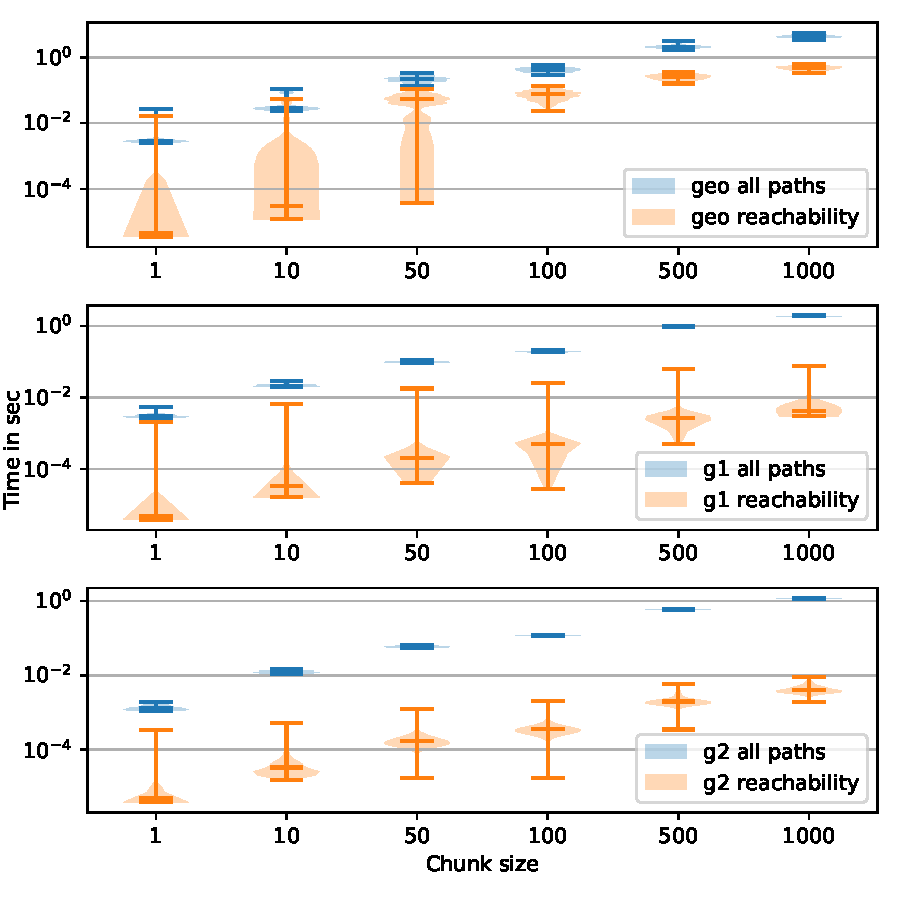
\includegraphics[width=0.5\textwidth]{geospecies_chunks.pdf}
    \caption{Multiple source CFPQ for \textit{Geospecies} graph and \textit{Geo} grammar: reachability and all paths}
    \label{fig:geo_multiple_source}
\end{figure}


First of all, we can see that the single-source queries are reasonably fast in both the \textit{reachability} and the \textit{all paths} cases: median time is less than $10^{-4}$ seconds for reachability queries, and is less than $10^{-2}$ seconds for \textit{all paths} queries. Even for queries $G_1$ and $G_2$, which return relatively small answers, time required for the all paths queries is bigger than for reachability queries. Moreover, time grows with the size of a chunk. Thus it is helpful to choose between the \textit{reachability} and \textit{all paths} modes to improve performance even for small start sets.

The median time is less than 1 second for all chunk sizes for the \textit{reachability} problem for the \textit{Geo} query. It is also true for the chunk sizes of less than 100 for the \textit{all paths} problem.

Comparison with CFPQ implementation for RedisGraph graph database~\cite{DBLP:conf/edbt/TerekhovPAZG21} shows that our solution is comparable with matrix-based algorithms. Note that our solution is sequential, while ReadisGraph uses SuiteSparse:GraphBLAS\footnote{SuiteSparse:GraphBLAS is a high performance implementation of GraphBLAS API in C language. Home page of project: \url{https://people.engr.tamu.edu/davis/GraphBLAS.html}. Accessed: 12.11.2021.} which is highly parallel. While the \textit{all pairs reachability} queries are slower for Neo4j, the \textit{multiple sources} queries for small chunks can be evaluated in comparable time. Moreover, our solution can compute all paths, while the solution for RedisGraph can solve only the reachability problem. Note that RedisGraph provides full stack support of CFPQ, so time for such steps as execution plan building is included into measured time, while we measure only query execution time  for Neo4j, omitting Cypher parsing, execution plan building, etc. 

Finally, we conclude that not only the linear algebra based CFPQ algorithms can be used in real-world graph analysis systems. It is not likely to outperform the linear algebra based CFPQ algorithms for the \textit{all pairs reachability}. But the GLL-based algorithm is promising for the \textit{multiple sources} queries with a relatively small start set, especially in the \textit{all paths} case. 